\documentclass[12pt, a4paper]{article}
\usepackage{amsmath}
\usepackage{amsfonts}
\usepackage{amsthm}
\usepackage{mathtools}
\newtheorem{theorem}{Theorem}[section]
\newtheorem{definition}{Definition}[section]
\numberwithin{equation}{section}
\usepackage{pgfplots}
\pgfplotsset{width=10cm,compat=1.9}
\graphicspath{ {img/} }
\DeclareGraphicsExtensions{.png}

\title{Convolutional Neural Networks}
\author{Kristian Wichmann}

\begin{document}
\maketitle

\section{Mathematical convolution}
In mathematics, the \textit{convolution} of two functions $f$ and $g$ is defined as:
\begin{equation}
(f*g)(t)=\int_{-\infty}^\infty f(\tau)g(t-\tau)\ d\tau
\end{equation}
By a change of variables $\sigma=t-\tau$, we have $\tau=t-\sigma$, and therefore $d\tau/d\sigma=-1$. Therefore:
\begin{equation}
(f*g)(t)=\int_\infty^{-\infty}f(t-\sigma)g(\sigma)(-d\sigma)=\int_{-\infty}^\infty f(t-\sigma)g(\sigma)\ d\sigma=(g*f)(t)
\end{equation}

\subsection{Discrete convolution}
If $f$ and $g$ are only defined on evenly spaced lattice points the integral in the convolution turns into a sum. Without loss of generality, we can assume these lattice points to be the integers:
\begin{equation}
(f*g)(x)=\sum_{\Delta x\in\mathbb{Z}}f(\Delta x)g(x-\Delta x),\quad x\in\mathbb{Z}
\end{equation}
We will only consider the case, where both $f$ and $g$ is non-zero for most values. Which means that the infinite sum will always be finite in practice, at least in this application.

In two dimensions, the functions are defined on $\mathbb{Z}\times\mathbb{Z}$ instead, and $x,\Delta x\in\mathbb{Z}\times\mathbb{Z}$ as well:
\begin{equation}
(f*g)(x)=\sum_{\Delta x\in\mathbb{Z}\times\mathbb{Z}}f(\Delta x)g(x-\Delta x),\quad x\in\mathbb{Z}\times\mathbb{Z}
\label{2d_convolution}
\end{equation}

This is the case we will use the most here.

\section{Filters and convolutions}

\subsection{Example: Edge detection}

\begin{figure}
\centering
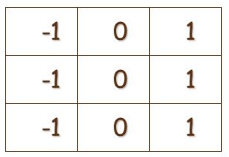
\includegraphics[width=0.4\textwidth]{horizontal_edge}
\caption{A filter for horizontal edge detection.}
\label{fig:horizontal_edge}
\end{figure}

Say we have a black and white image represented in an array of pixel values. If we want to detect horizontal edges, we can think of this as determining the pixel value gradient in the $x$ direction. This should be done all over the picture. One such way to do this, is to look at the immediate neighborhood of pixel value around each point in the picture, i.e. nine pixels in total. Then multiply them by the numbers in the $3\times 3$ matrix shown in figure \ref{fig:horizontal_edge}, and add up all nine values as shown by figure \ref{fig:convolutional_filter}. This will be an approximation to the gradient in the $x$ direction (the opposite of figure \ref{fig:horizontal_edge}, though) in the vicinity of the middle pixel as desired (or at least proportinal to it). In figure \ref{fig:convolutional_filter} we see that overall, the gradient is to the right, which the negative result reflects.

\begin{figure}
\centering
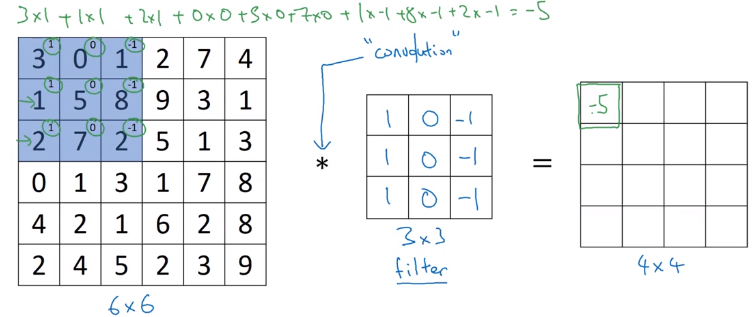
\includegraphics[width=\textwidth]{convolutional_filter}
\caption{How convolution works.}
\label{fig:convolutional_filter}
\end{figure}

For a $n\times n$ image, we can repeat this process for $(n-2)\times(n-2)$ sets of $3\times 3$ blocks of pixels. So the results of the convolution can be represented as an image slightly smaller than the original. Below we will look at how we can avoid this shrinkage.

\subsection{General filter}
There is nothing special about the number in the filters we've used in the edge detection example above. In fact, a central idea in convolutional neural networks is for the algorithm to learn the values of a filter. These are also sometimes known as \textit{kernels}.

Also filter need not be $3\times 3$. It can have any size, but square with an uneven number of pixels on each side is the most common.

\subsection{Padding}
The procedure above is very similar to the mathematical discrete convolution described in equation \ref{2d_convolution} with $f$ being the filter and $g$ being the image\footnote{Strictly speaking, the image (or equvalently the filter) should be reversed in both axes according to the mathematical definition. The operation we've described is known as \textit{cross-correlation}. But here, we will simply refer to it a convolution.}. But of course neither of these are of infinite size as the equation requires. Instead we can think of the remaining, infinite number of values to be zero. And we then only consider the non-trivial output window.

But this actually gives ud a way to avoid the image size shrinkage inherent to filtering: As we saw above, a $n\times n$ image convoluted by an $f\times f$ filter results in an output of size $(n-f+1)\times(n-f+1)$. However, if we pad the input image with zeros in all directions, we can avoid this problem. If we pad by $p$ zeros in all four directions, we now get a new input size of $(n+2p)\times(n+2p)$. We want an output size of $(n-f+1)\times(n-f+1)$ as before:
\begin{equation}
n+2p=n-f+1\Leftrightarrow p=\frac{f-1}{2}
\end{equation}
So we will need a margin of zeroes of thickness $p=(f-1)/2$ to keep the image size. Here we see why $f$ is usually chosen to be odd.

Having no padding is sometimes knows as a \textit{valid} convolution, while padding to preserve image size as described above is called a \textit{same} convolution.

\subsection{Stride}
So far, we've used a \textit{stride} $s$ of 1, which means that every time we've moved the convolutional filter we've moved it a single pixel. But we might as well have moved it two or more pixels (both directions). The amount moved is the stride.

With stride 1, an input size of $n\times n$ with padding $p$ results in an output of $n+2p-f+1$ as shown above. But when we move $s$ pixels at a time, we have to divide by $s$ for an output size of:
\begin{equation}
\frac{n+2p-f}{s}+1
\end{equation}
Now, what happens if the fraction is not an integer? In that case, we miss the "last" point. So we have to take the integer part, i.e. rounding down:
\begin{equation}
\left\lfloor\frac{n+2p-f}{s}\right\rfloor+1
\end{equation}

\section{Convolution of multiple channels}
An image is typically not black and white, but has colors. This means that is has three \textit{channels}, namely red, green, and blue, or RGB. This is notated as a seperate dimension. So such a color image of height 300, width 200 would have dimensions $200\times 200\times 3$.

Similarly, if we want to apply a filter for convolution, there must be a matrix of numbers for each channel. So a 5 by 5 pixel filter on a RGB image would have dimensions $5\times 5\times 3$. Because the convoutional sum is now over three dimensions, the output will be two-dimensional. For instance if a $100\times 100\times 3$ image is convoluted by a $5\times 5\times 3$ filter, we would get a $96\times 96$ "image" as output (remember the $n-f+1$ formula).

Now, image we have $n$ such filters. Then we may collect all the two dimensional outputs into a new three dimensional object. For instance, if we had 10 filters in the example above, we would end up with a $96\times 96\times 10$ object as output. I.e. the number of filters in one layer is equal to the number of channels in the next.


\end{document}